\documentclass{article}

\usepackage{amsmath}
\usepackage{gensymb}
\usepackage{graphicx}
\usepackage{caption}

\title{On the Properties of Solenoid Originated Magnetic Fields}
\author{Elliott Ashby}
\date{\today}


\begin{document}
    \maketitle
    
    \section{Introduction}
    
    \subsection{Aim}
    This small project aims to investigate some of the properties of 
    solenoid originated magnetic fields in a Helmholtz Pair configuration investigating magnetic field neutralisation 
    along with investigation of the magnitudes of the magnetic field on a non symmetrical axis to a single solenoid.
    \newline This will be accomplished with a combination of theoretical 
    calculations along with experimental evidence in order to prove that Biot-Savart Law is valid for all axis relative to a solenoid of origin.
    \subsection{Methods}
    \subsubsection{Neutralising Magnetic Fields}
    \begin{enumerate}
        \item Zero hall monitor agaist earths magnetic fields.
        \item Position two solenoids 20cm apart. Such as in \textbf{Figure 1}.
        \item Reverse current connections on one of the solenoids in order to reverse the direction of the magnetic fields.
        \item Set power supply to 1.5A.
        \item In a systematic manner, vary the hall probe along the common axis of the solenoids and record the magnetic field in Gauss and the distance from a solenoid of one's choice.
        \item Plot Gauss against distance z (cm).
    \end{enumerate}
   \subsubsection{Alternate Axis Measurements from a Single Solenoid}
   \begin{enumerate}
       \item Zero hall monitor against earth's magnetic fields.
       \item Set up a single solenoid at 1.5A.
       \item Vary the hall probe's distance along the x axis 90\degree from C (C=13cm on the z axis for our measurements) as seen in \textbf{Figure 2}.
       \item Record hall effect in Gauss and distance x in cm.
       \item Plot Gauss against distance x (cm).
   \end{enumerate}
   \begin{figure}
       \centering
       \includegraphics[scale=0.56]{/home/tex/images/scrots/2021-12-07-00:30:10-screenshot.png}
       \caption{A Helmholtz pair}
   \end{figure}
   \begin{figure}
       \centering
       \includegraphics[scale=0.9]{/home/tex/images/scrots/2021-12-07-00:35:01-screenshot.png}
       \caption{Alternate Axis Setup}
   \end{figure}
   
   \section{Results}
   \subsection{Neutralising Magnetic Fields}
%    \begin{figure}
%        \centering
%        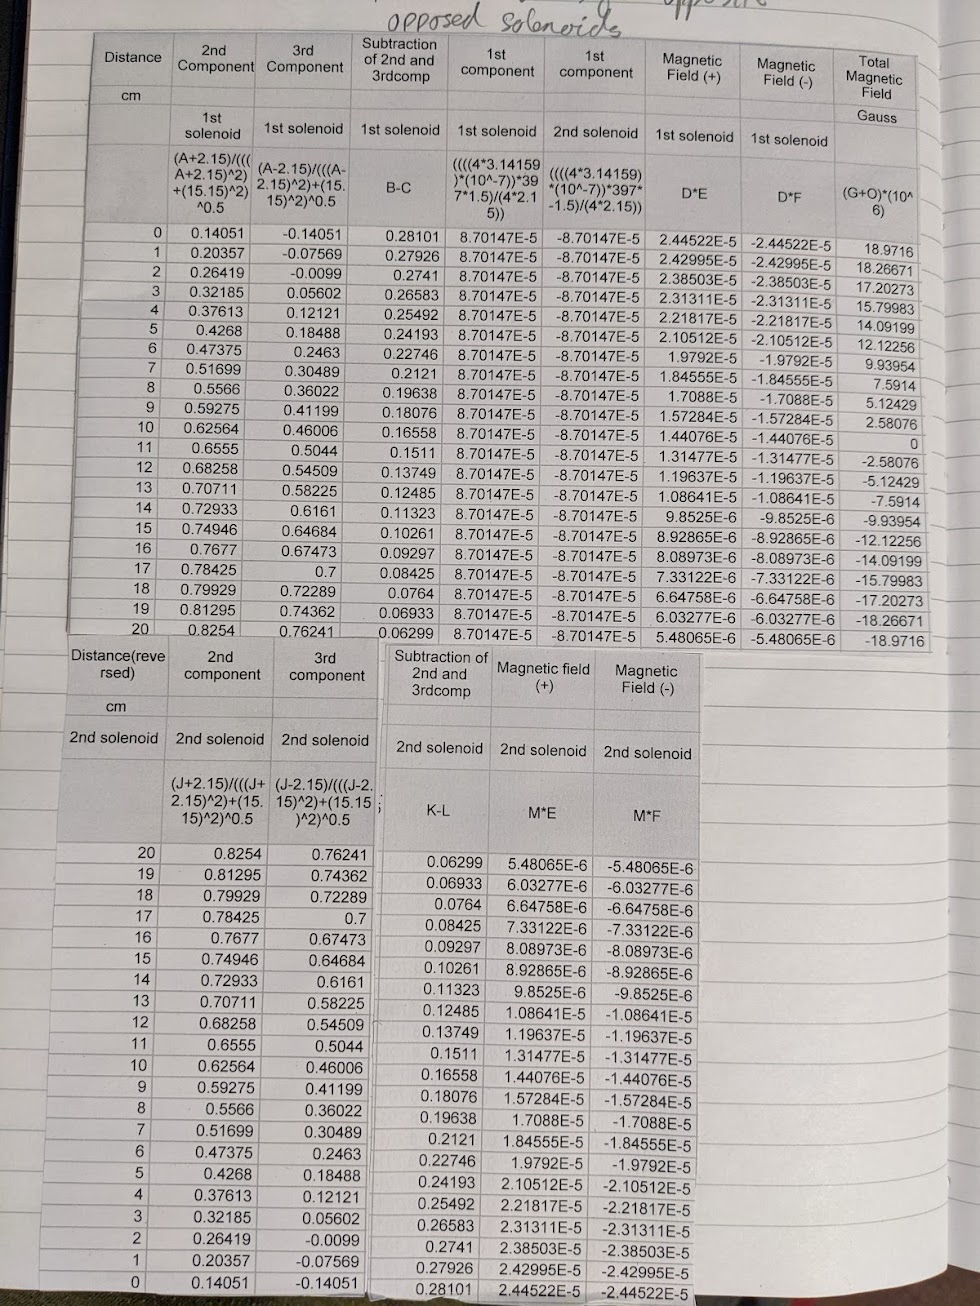
\includegraphics[scale=0.3]{/home/tex/Documents/Work/physics/latex/media/images/theorysol.jpg}
%        \caption{Theoretical Values for Neutralising Magnetic Fields}
%    \end{figure}
   \begin{figure}
       \centering
       \includegraphics[scale=0.6]{/home/tex/images/scrots/2021-12-07-00:30:45-screenshot.png}
       \caption{Graphing Theoretical Magnetic Field in Gauss against z distance in cm}
   \end{figure}
%    \begin{figure}
%        \centering
%        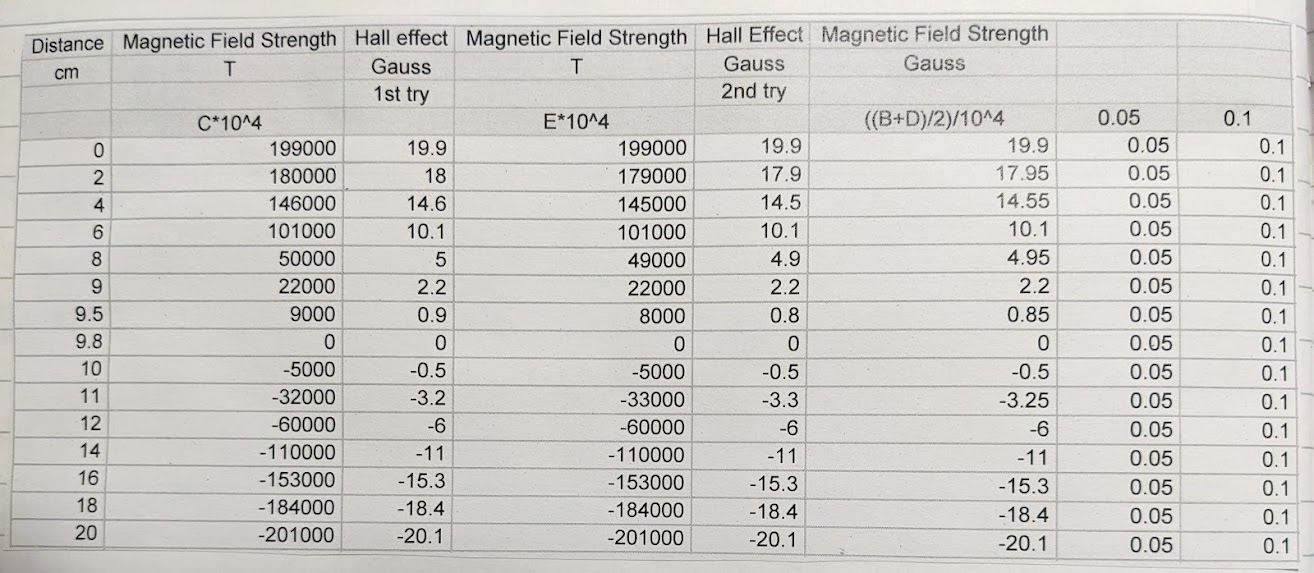
\includegraphics[scale=0.3]{/home/tex/Documents/Work/physics/latex/media/images/expres.jpg}
%        \caption{Experimental Values for Neutralising Magnetic Fields}
%    \end{figure}
   \begin{figure}
       \centering
       \includegraphics[scale=0.6]{/home/tex/images/scrots/2021-12-07-00:30:34-screenshot.png}
       \caption{Graphing Experimental Magnetic Field in Gauss against z distance in cm}
   \end{figure}
   The magnetic fields generated by the opposed solenoids can be seen in \textbf{Figure 3}
   creating a system of magnetic fields between the 2 solenoids that oppose each other. The theoretical values can be calculated
   with the \textbf{Biot-Savart Law};
   \begin{equation}
       d{\bf{B}} = \frac{{\mu _0 }}{{4\pi }}\frac{{Id\ell \times {\bf{\hat r}}}}{{r^2 }}
   \end{equation}
   \textbf{B} in (1) is measured in Tesla, so in order to compare it to our experimental values, we converted it to Gauss by
   multiplying by 10\textsuperscript{4}. \newline
   In order for a calculation to be done on a coil like those found in a Helmholtz pair in order to find magnetic field strength at 
   distance z from the centre of one of the coils, the Biot-Savart Law is derived into equation (2) where I is the current, \(\mu\)\textsubscript{0} is the permeabilty 
   constant and N are the number of loops in the solenoid.
   \begin{equation}
       B_z = \frac{\mu _0 N I}{A \ell}\bigg( \frac{z + \ell}{\sqrt{(z + \ell)^2 + R^2}} - \frac{z - \ell}{\sqrt{(z - \ell)^2 + R^2}}\bigg)
   \end{equation}
   Using known values of N = 397, I = 1.5A, \(\ell\) = 2.15cm and R = 15.15cm the theoretical values can be calculated for all values of z, allowing us to plot the same
   values as those we measure experimentally, these results can be seen in \textbf{Figure 3} and \textbf{Figure 4}
   \subsubsection{Expected Results}
   The results expected from this experiment are as follows
   \begin{itemize}
       \item The same magnitude of magnetic field at distances 0cm and 20cm.
       \item Manetic field 0 Gauss at 10cm.
       \item Opposing quadratic relationships "added" together to create a cubic relationship since the magnetic field strength varies like \(\frac{1}{r^2}\).
   \end{itemize}
   These critical features can clearly be seen in theoretical values calculated seen graphed in \textbf{Figure 3}.
   \subsubsection{Observed Results}
   From experimental values shown in \textbf{Figure 4}, these features can clearly be identified in relation to the expected model, however, accounting
   for standard uncertainty represented in the curve fit, some aspects are still far from theoretical values. These aspects and possible explanations include;
   \begin{itemize}
       \item Different values at 0cm and 20cm \(\rightarrow\) This arises from the two solenoids generating different magnetic fields from the same current supply,
       as seen from \textbf{Figure 3}, a differance of 0.2 Gauss in magnitude can be observed, with the solenoid generating a more powerful magnetic field
       being the one located at 20cm. This may be for a variety of reasons such as different number of loops, higher density of loops or lower resistance.
       \item The experimental difference referenced above also affects a non 0 Gauss measurement at 10cm \(\rightarrow\) Due to the difference in generated magnetic fields
       and the solenoid located at 20cm being stronger at the same current of 1.5A, instead of the magnitudes of magnetic field being equal at equal radius, they are instead 
       different by 0.5 Gauss bias toward the solenoid located at 20cm. This means that the actual location of equilibrium of the magnetic fields is at 9.8cm instead of 10cm.
       \item Another inconsistency is in the absolute values when compared to theoretical values, most easily seen at 0cm and 20cm, where comparing theoretical against experimental yields 
       differences from the expected 18.97 Gauss where the solenoids at 0cm generate a magnitude of 19.9 Gauss and at 20cm generate a magnitude of 20.1 Gauss. \(\rightarrow\) If you consider 
       an average of the two experimental values at 20 Gauss, this is roughly 1 Gauss higher than the expected theoretical value. While we are unsure as to what definitively caused this difference 
       since 1 Gauss difference is much larger than the uncertainty maximum of \(\pm\)0.11 Gauss one can speculate that this difference is perhaps due to other factors such as greater unmeasurable inaccuracies
       in the hall probe or miscalculations in the hall voltage to gauss automated calculations not under our control.
   \end{itemize}
   Focusing now on the similarities;
   \begin{itemize}
       \item Experimental results yielded values and relationships extremely similar to theoretical values (\textbf{Figure 3, Figure 4}), both boast a negative cubic relationship 
       formed from the difference of two \(\frac{1}{r^2}\) relationships.
       \item The polynomial curve fits of \textbf{Figure 3} and \textbf{Figure 4} have similar coefficients, the largest difference being the coefficient of x at 0.08, however this is only 6.625\% of the average of the 
       two coefficients. Considering other inaccuracies that cannot be measured due to our setup, this is a reasonable difference of fits such that their similarity can be noted.
   \end{itemize}
   \subsection{Alternate Axis Measurements from a Single Solenoid}
   This experiment aims to prove that the Biot-Savart Law is valid for not only the z axis but for other axis as well. The setup for this can be seen in \textbf{Figure 2}
   where the hall probe will be varied along the y axis in order to measure the magnetic force generated by a single coil.
   \begin{figure}
       \centering
       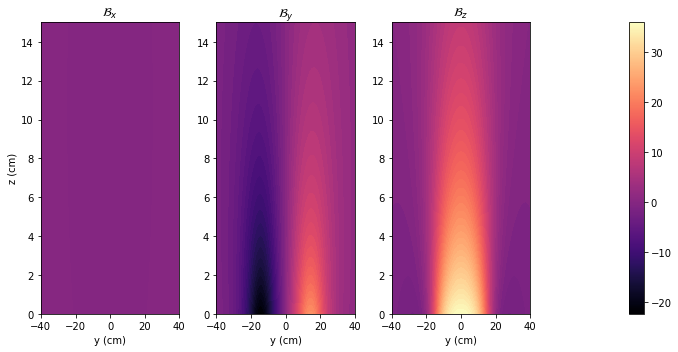
\includegraphics[scale=0.5]{/home/tex/Documents/Work/physics/latex/media/images/heatmap.png}
       \caption{Heatmap of components of the theoretical magnetic field strength (Gauss) of a single coil in the y-z plane.}
   \end{figure}
   \begin{figure}
        \centering
        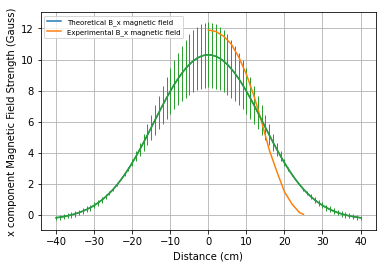
\includegraphics[scale=0.9]{/home/tex/Documents/Work/physics/latex/media/images/theoryvsexper.png}
        \caption{Plot of theoretical vs experimental values at z = 13cm, theoretical values have error bars of \(\pm\)1cm in the z axis.}
   \end{figure}
   \begin{figure}
       \centering
       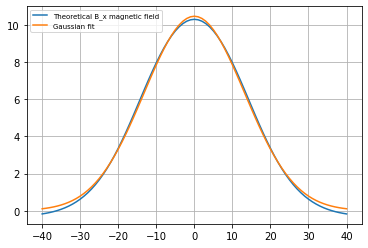
\includegraphics[scale=0.9]{/home/tex/Documents/Work/physics/latex/media/images/theoryvsgauss.png}
       \caption{Theoretical values at z = 13cm plotted with a gaussian fit of the same data set.}
   \end{figure}
   \subsubsection{Expected Results}
   Expected results for this experiment are slightly harder to pin down, as multiple values are now being varied. This is because while the increase in radius would
   suggest the magnitude will fall like \(\frac{1}{r^2}\) the magnetic flux now passes through the hall probe at angle \(\tan^-1(\frac{y}{+C\hat{z}})\). So expected results 
   seem likely to follow the inverse square law along with a correction with a tan\(\theta\) factor to find the magnitude of components.
   \subsubsection{Observed Results}
   \textbf{Figure 5} shows a heat map across the z-y plane with the intensity of the heat map being equal to the magnitude of the magnetic field in Gauss for all three components. These were calculated 
   using python and matplotlib plotting libraries along with the Biot-Savart Law [Equation (1)].
   \newline Using this large matrix of values, any cross section can be taken to compare against experimentally found data.
   \newline This is what \textbf{Figure 6} shows, along with error bars generated from z = 13\(\pm\)1cm since the true position of the hall monitor within 
   it's encasement is unknown and may vary by up to 2cm.
   \newline
   \newline
   \textbf{Figure 6} shows a clear similarity between observed experimental values and theoretical ones with a similar relationship. Despite this some clear differences are present
   such as the peak magnitude at 0cm and the rate of decrease in the magnetic field strength along with the point where 0 Gauss is reached. Even though there are some differences in the curves, 
   the similarity in the relationship is shown as when the theoretical values are calculated closer to z = 14cm, the first half of the curves, up to around 15cm (incidentally, the radius of the solenoid is 15.15cm)
   where the two curves diverge as they approach 0.
   \newline Some possibilities to the differences between experimental values and theoretical ones are as follows;
   \begin{itemize}
       \item Larger inaccuracies in experimental results than expected, possibly due to factors such as, the measurements not being precisely 90\(\degree\) to the z axis causing a greater drop at lower y distances as the true radius would be larger than expected.
       \item There is a possibility that the values of the properties of the coil provided are incorrect or inaccurate.
       \item Incorrect simulated theoretical results.
   \end{itemize}
   \textbf{Figure 7} shows the same theoretical values as in \textbf{Figure 6} in addition to a gaussian curve represented as;
   \begin{equation}
    X \sim \mathcal{N}(\mu,\,\sigma^{2})\,.
   \end{equation}
   and calculated from;
   \begin{equation}
    {\displaystyle f(x)={\frac {1}{\sigma {\sqrt {2\pi }}}}e^{-{\frac {1}{2}}\left({\frac {x-\mu }{\sigma }}\right)^{2}}}
   \end{equation}
   The theoretical values for the x component of magnetic field strength generated from a single coil, form a closely approximated gaussian distribution.
   \newline Performing a \(\chi^2\) goodness of fit test using;
   \begin{equation}
    \chi^2=\sum \frac{(O - E)^2}{E}
   \end{equation}
   gives a result of \(\chi^2 \approx 0.73\) indicating that the distribution in \textbf{Figure 7} 
   is indeed extremely close to a true gaussian distribution.
   \newline
   \newline
   I believe this relationship to be formed due to the hall probes orientation. As the probe continues to increase its distance in the y direction, while maintaining the same orientation and 
   z value, the angle between the radius vector and the z axis continues to increase at a decreasing rate. This will result in the rate of change of magnetic flux with respect to distance to decrease
   for larger values of y.
   \section{Conclusions}
   Following the aims of the experiments, the Helmholtz Pair acted as expected, following expected theoretical values in relationship very closely
   with a maximum deviation of 6.625\(\%\) from theoretical values. Further experiments to extend this would be along the lines of ivestigating at different coil separation distances
   along with varying the current in one or both of the coils.
   \newline
   Using the results from the Alternate Axis Measurements from a Single Solenoid experiment. 
   We can conclude that the Biot-Savart Law is valid for all axis relative to a solenoid of origin. This is because, the relationship shown experimentally matches that which was calculated 
   from the Biot-Savart Law.
   \newline
   \newline In addition, it was shown that along the y axis the magnetc field varies as gaussian distribution with a \(\chi^2 \approx 0.73\) when compared to a true gaussian distribution.

   \begin{theindex}
       \item \textbf{Figure 1 \& 2:}
       \subitem Yousad, Adnan \& Khan, Fatimah \& Reindl, Leo. (2011). Wireless sensing of open loop micro inductors using Helmholtz coil. International Journal on Smart Sensing and Intelligent Systems. 4. 527-546. 10.21307/ijssis-2017-455
        \item \textbf{Figure 5:}
        \subitem Elliott Ashby. (2021). Biot-Savart python library (Mingde Yin and Ryan Zazo) rewritten for python 3.9.9, Plotting from matplotlib
    \end{theindex}
\end{document}